\renewcommand{\thefootnote}{\fnsymbol{footnote}}

\newcommand{\Bulk}{B_0}
\newcommand{\BPrime}{{B'_0}}

\documentclass[prb,aps,nobibnotes,twocolumn,doublespace,twocolumngrid,superbib]{revtex4}
%\documentclass[prb,aps,nobibnotes,superbib,preprint]{revtex4}

\usepackage{graphicx}
\usepackage{amsfonts}
\usepackage{bm}
\usepackage{alltt}
\usepackage{dcolumn}
\usepackage{amsmath}
\usepackage{graphicx}
\makeatletter
\makeatother

\begin{document}
\title[Short Title]{ 
All-electron density functional studies of hydrostatic compression of 
pentaerythritol tetranitrate (PETN)}
\author{Chee Kwan Gan\footnotemark[1]}
\author{Thomas D. Sewell\footnotemark[2]}
\author{Matt Challacombe\footnotemark[3]}

\affiliation{ Theoretical Division, Los Alamos
              National Laboratory,\\ Los Alamos, New Mexico 87545}
\date{Oct 29, 2003}

\begin{abstract}
All-electron calculations of the hydrostatic compression of
pentaerythritol tetranitrate (PETN) crystal have been performed using
density functional theory with the PBE functional in conjunction with
the 6-31G** Gaussian basis set.  Full optimizations of the atomic
positions and ratio of lattice parameters $c/a$ for the tetragonal
crystal were performed for eight volume ratios $0.65
\le V/V_0 \le 1.00$, where $V_0$ is the equilibrium volume at zero
pressure.  The pressure, linear compressibilities of lattice
parameters $a$ and $c$, and $c/a$ ratio as functions of volume ratio
are in good agreement with experiment.  It is observed that
$c/a$ decreases monotonically with compression until $V/V_0=0.8$, 
and then increases monotonically for all higher levels of compression
considered.  Changes in intramolecular coordinates
and close intermolecular contact distances were studied as a function
of compression.  The results indicate essentially rigid-molecule compression
for $V/V_0 >0.8$, with the onset of significant intramolecular distortion
for higher compressions.  Predictions of the bulk modulus $\Bulk$ and its 
pressure derivative $\BPrime$ were obtained using various equation of 
state fitting forms. Values for these quantities are compared to 
experiment and to the results of a preceding molecular simulation study 
of PETN based on an empirical force field.

\smallskip
\noindent{\bf Keywords}: Density functional theory, linear scaling, 
Gaussian-Orbital, PETN, hydrostatic compression
\end{abstract}

%\pacs{31.15.-p; 31.15.Ew; 02.60.Jh}
\maketitle

\footnotetext[0]{Preprint LA-UR-03-5336.}
\footnotetext[1]{\tt CKGan@LANL.Gov}
\footnotetext[2]{\tt Sewell@LANL.Gov}
\footnotetext[3]{\tt MChalla@LANL.Gov}

\section{Introduction}
Pentaerythritol tetranitrate [PETN, C(CH$_2$ONO$_2$)$_4$] is an
important secondary high explosive.  At room temperature, PETN
crystallizes in a tetragonal space group, P$\bar{4}$2$_1$c, with two
molecules per unit
cell.~\cite{Booth_1947v,Trotter_1963v16,Conant_1979} A
high-temperature form denoted PETN-II has also been
reported.~\cite{Cady_1975vB41} PETN has received a lot of attention
due to interesting anisotropic, non-monotonic shock initiation
sensitivity.~\cite{Dick_1984v44,Dick_1991v70,Gallagher_1992v339,Dick_1997v81,Gruzdkov_2000v104,Yoo_2000v88}
The room temperature linear and volumetric hydrostatic compression of
PETN has been measured by Olinger and
co-workers~\cite{Olinger_1975v62,Olinger_1976} using x-ray diffraction
for pressures up to 10.45~GPa.  Dick and von Dreele~\cite{Dick_1997}
used neutron scattering from deuterated PETN to study detailed
pressure-induced changes in dihedral angles and molecular orientations
in the unit cell for pressures up to 4.28~GPa.
While the volumetric compression reported by Dick and von Dreele is
consistent with the data of Olinger {\it et al.}, significant
differences are observed in the linear compressions along the $a$ and
$c$ crystal axes.

A complete set of isentropic elastic coefficients for PETN has been
reported by Morris~\cite{Morris_1976} based on extensive single
crystal sound speed measurements.  The resulting elastic tensor was of
high precision with the exception of element $C_{13}$, which had an
uncertainty over ten times the average for the others.  Winey and
Gupta~\cite{Winey_2001v90} re-analyzed Morris' data, identified the
source of the inconsistency in $C_{13}$, and reported an internally
consistent and precise elastic tensor.

There have been a number of theoretical studies of PETN crystals based
on empirical force fields.  Dick and
Ritchie~\cite{Dick_1994v76} performed molecular mechanics calculations
using the AMBER4.0 force field to study the energetics associated with
slip along specific directions in the crystal, in an effort to
understand the anisotropic initiation sensitivity in PETN.  Their
results were largely consistent with experimental data, but were not
conclusive due to the lack of rate-dependent information.

Theoretical predictions of PETN crystal structure, thermal expansion,
and hydrostatic compression were reported by Sorescu {\it et
al.}~\cite{Sorescu_1999v103A, Sorescu_1999v103} They used an
intermolecular potential function developed in their laboratory
in conjunction with a rigid-molecule 
approximation for the molecular structure. Agreement to within one percent 
of experiment was obtained for the crystal lattice parameters at 298~K, although
the calculated thermal expansion coefficient was three times smaller than the
experimental value.  Sorescu {\it et al.}~\cite{Sorescu_1999v103}
predicted linear compressibilities that were in reasonable agreement
with experiment for pressures below 6~GPa, with the onset of
significant discrepancies for higher pressures.  (The calculated
linear compressibilities were systematically lower than the measured
ones, resulting in a larger error in the volumetric compressibility
over the entire pressure interval, and leading to a 41\% error
compared to experiment in the predicted initial bulk modulus.) The
authors attributed the errors in their predictions at higher pressure
to a shortcoming of the rigid-molecule approximation.

Bunte and Sun~\cite{Bunte_2000v104} reported a flexible molecule
inter- and intramolecular COMPASS force field parameterization based
on a calibration to experimental data and high level gas phase
electronic structure results for selected nitrate esters.  Although
PETN was not part of the force field training set, predicted crystal
lattice parameters for PETN were in good agreement with experiment.
Bunte and Sun reported five of the six elastic coefficients for PETN
at zero Kelvin, based on energy-minimized lattice parameters as well
as for a constrained calculation in which the lattice parameters were
set equal to experimental values.  Reasonable agreement with
experimental data was obtained in the latter case, in spite of neglect
of explicit thermal effects.  Since they did not report the $C_{13}$
elastic coefficient, it is not possible to obtain a bulk modulus from
their work.

Zaoui and Sekkal~\cite{Zaoui_2001v118} reported calculations of PETN
thermal and mechanical properties using a flexible molecule, Tersoff-like force
field.  This work is difficult to interpret, as the primary simulation
cell described in the article corresponds to a non-integral number of
molecules, and the predicted longitudinal and transverse sound speeds
are both unrealistically small and inconsistent with the reported bulk
modulus.  For these reasons, it will not be considered further below.

Kuklja and Kunz~\cite{Kuklja_2001v89} studied the electronic structure 
of PETN crystal containing an edge dislocation using Hartree-Fock
theory with CRYSTAL95/98.~\cite{Crystal95} They considered
edge-type dislocations with Burgers vector [001], and 
found that a shear stress, induced by the dislocations, produces local 
electronic states in the fundamental band gap of the crystal.

In this contribution, we report condensed phase electronic-structure
calculations of the hydrostatic compression of PETN at absolute zero
and pressures up to 25~GPa.  We employ an all-electron
density-functional method using the PBE~\cite{Perdew_96v77} functional
in conjunction with the 6-31G** Gaussian basis set.  Complete
optimization of the cell contents and $c/a$ ratio of the lattice
parameters is performed at each of the eight volumes considered,
assuming a tetragonal cell (i.e., $a=b \neq c$,
$\alpha=\beta=\gamma=90^\circ$).  It should be noted that our
all-electron treatment is computationally more demanding than
pseudopotential methods, but it should be free from potential errors
associated with pseudopotentials that may become important at high
pressures.

The remainder of this paper is organized as follows: In
Section~\ref{sec:comput} we describe the computational framework and
in Section~\ref{sec:protocol} the details of our calculations. In
Section~\ref{sec:results} we present the results of the calculations
and properties derived from them, with comparisons to experiment and
previous theoretical studies.  Finally, in
Section~\ref{sec:conclusions} we summarize the main conclusions of our
work.

\section{Computational Framework}
\label{sec:comput}
Calculations were performed using a parallelized version of
MondoSCF,~\cite{MondoSCF} a suite of programs for linear scaling
electronic-structure theory and {\it ab initio} molecular dynamics.
Periodic boundary conditions~\cite{CTymczak03} were used to study the
PETN crystal.  The MondoSCF code employs a number of advanced ${\cal O}(N)$
techniques such as the quantum chemistry tree code (QCTC) for the
Coulomb matrix
build~\cite{MChallacombe96,MChallacombe96B,MChallacombe97} and the
adaptive Hierarchical Cubature (HiCu) for the exchange-correlation
matrix build.~\cite{MChallacombe00A} Parallelization of MondoSCF has
been carried out, where an exemplary success is the efficient
data-parallel algorithm for the HiCu method~\cite{CGan03} with an
equal-time partitioning scheme that exploits the temporal locality of
SCF calculations to achieve excellent load balance.  
We used a cluster of 256 4-CPU HP/Compaq Alphaserver ES45s with the Quadrics 
QsNet High Speed Interconnect to perform the calculations in this work.  
Most calculations were performed using 32 processors.

\section{Computational Protocol}
\label{sec:protocol}
The results described below are for three-dimensionally periodic,
gradient-corrected density-functional theory (GGA), using the PBE
functional~\cite{Perdew_96v77}. The small 3-21G split-valence Gaussian 
basis set was tried first, but found to be inadequate relative to the
larger 6-31G** basis set.  Thus, the 6-31G** basis set was used
for all results reported here. The $\Gamma$-point for Brillouin zone sampling was 
used throughout with the crystallographic unit 
cell, which contains two molecules (58 atoms).  However, a number of calculations 
were carried out using a $1 \times 1 \times 2 $ supercell to verify 
convergence of the $\Gamma$-point approximation (as shown in 
Fig.~\ref{fig:volume_compress}(a)).  
Because of the necessity to resolve milihartree energy differences,
a ``good'' level of numerical approximation was used throughout to
achieve the required 7-8 digits of accuracy in the total energy,
which was approximately $-$2600 Hartree.
This combination of large basis set and accurate numerical
approximation was mastered through parallel ${\cal O}(N)$ algorithms, a 
key enabling technology for these types of calculations. 

Starting with the experimental x-ray crystal structure reported by
Conant {\it et al.},~\cite{Conant_1979} we calculated the zero
pressure unit cell volume $V_0$ under the assumption of a tetragonal
lattice ($a=b\neq c$, $\alpha=\beta=\gamma=90^\circ$) by computing
fully energy-minimized structures on a $5\times 5$ grid of $a$ and $c$
lattice parameters, and fitting the results to a cubic polynomial in
$a$ and $c$.  A subsequent calculation on a $3 \times 3$ grid centered
at the minimum predicted from the preceding step was used to obtain an
improved prediction of the optimized crystal structure.  These
correspond to $a_0$, $c_0$ and $V_0=a_0^2c_0$.  Stability of the 
tetragonal structure was checked by energy minimization of nearby
orthorhombic structures ($a\neq b\neq c$) in the vicinity of the tetragonal 
minimum; these tests confirmed that the tetragonal structure is favored 
energetically over neighboring orthorhombic ones.

Energy-minimized structures for a given volume ratio $V/V_0$ were
obtained by scanning a set of $c/a$ ratios consistent with the desired
volume $V$.  Initial guesses were obtained by rigid translation of the
molecular structure obtained from the next larger volume ratio via a
transformation that preserves the center-of-mass positions in
crystallographic coordinates.  Typically, seven values of $c/a$ were
considered at a given volume, and the results were fit to a parabola.

\section{Results}
\label{sec:results}
Calculated and measured lattice parameters are compared in
Table~\ref{tab:table1}, where we also include the experimental results
of Olinger {\it et al.}~\cite{Olinger_1975v62} and Conant {\it et
al.}~\cite{Conant_1979}, and the theoretical predictions of Sorescu
{\it et al.}~\cite{Sorescu_1999v103} and Bunte and
Sun~\cite{Bunte_2000v104} for completeness.  Percent errors in our
calculations relative to the experimental results of Conant {\it et
al.}~\cite{Conant_1979} are 0.51\%, 0.75\%, and 1.8\% for $a_0$,
$c_0$, and $V_0$, respectively.  It is important to note, however,
that we have not attempted to correct for thermal expansion, since
experimental coefficients of thermal expansion for PETN do not extend
to cryogenic temperatures.

Calculated intramolecular coordinates and selected intermolecular
distances are compared to the experimental results of Conant {\it et
al.}~\cite{Conant_1979} in Table~\ref{tab:table2} (see also 
Fig.~\ref{fig:petn_2d}).  The predicted
molecular geometry is in excellent agreement with experiment.  The
12\% discrepancy in the C-H distances is expected, since we are
comparing to x-ray data.  Otherwise, most of the intramolecular
degrees of freedom are accurately predicted to within a few percent.
There are three intermolecular distances less than 3~\AA\ at
equilibrium, each of which is an O$\cdot\cdot\cdot$H contact.
Predicted values are 2.396~\AA, 2.779~\AA, and 2.898~\AA, with errors
relative to experiment of $-$3.5\%, $-$0.7\%, and 0.1\%, respectively.

The volumetric hydrostatic compression is summarized in
Fig.~\ref{fig:volume_compress}.  The variation of the energy with
volume ratio is shown in Fig.~\ref{fig:volume_compress}(a).  The line
is a sixth degree polynomial fit, from which the pressure shown in
Fig.~\ref{fig:volume_compress}(b) is obtained as $P=-dE/dV$.  The open
circles in Fig.~\ref{fig:volume_compress}(b) are the experimental data
of Olinger {\it et al.}, with experimental uncertainties comparable to
the symbol sizes.  The calculated volumetric compression is in
remarkably good agreement with experiment.  The effects of temperature
would be expected to ``soften'' the calculated isotherm at low
pressures;  however, this effect should diminish quickly with
increasing compression. While perhaps obvious, it is worth pointing out
that this behavior has been observed for similar systems, including 
$\beta$-octahydro-1,3,5,7-tetranitro-1,3,5,7-tetrazocine
($\beta$-HMX)\cite{Gump_2003,Sewell03_unpublished}.

The linear compression along the $a$ and $c$ crystallographic
directions is shown in Fig.~\ref{fig:linear_compress}.
Figure~\ref{fig:linear_compress}(a) reveals good agreement between our
predictions and the experimental data for the relative compressions of
$a/a_0$ and $c/c_0$.
In Fig.~\ref{fig:linear_compress}(b) we show the variation of the
$c/a$ ratio as a function of compression.
The solid line is based on polynomial representations of $a=a(V)$ and
$c=c(V)$ due to Olinger {\it et al.}~\cite{Olinger_1975v62} We observe
in both cases an initial decrease in the $c/a$ ratio with increasing
compression, followed by an increase toward a more ``cubic-like''
lattice structure.  The positions of the minima in the curves are in
fairly good agreement, and correspond to a volume ratio of 0.8 and a
pressure of about 7~GPa.

In Figs.~\ref{fig:intramolecular}(a) and (b), we show the changes in
intramolecular bond lengths and three-center angles as PETN is
compressed.  For clarity of presentation, we only include coordinates that
undergo significant changes.  It is observed that the bond lengths and angles
remain almost constant for $ 0.8 \leq V/V_0 \leq 1.0$, with the onset of
sizable changes for higher compressions.  Backbone dihedral angles (not shown)
exhibit qualitatively similar behavior, with changes of 2--5 degrees beginning
at $V/V_0=0.8$. (We note that Dick and von Dreele~\cite{Dick_1997} observed
nonmonotonic variations of up to several degrees in some of the dihedral
angles in deuterated PETN between zero and 4.28~GPa.  We do not see any
evidence for this in our calculations, based on the four compressions in
our study that correspond to this pressure interval.)
Figure~\ref{fig:intramolecular}(c) depicts the pressure response of 
the three sets of intermolecular van der Waals contacts that are below 
3~\AA\/ at zero
pressure; each of these corresponds to an O$\cdot\cdot\cdot$H
interaction.  The two longer distances decrease essentially linearly
over the entire interval of compression studied, whereas the shorter
one exhibits an obvious change in slope at about $V/V_0=0.8$, which we
again note is the volume ratio corresponding to the minimum in $c/a$.


The results in Fig.~\ref{fig:intramolecular} are consistent with the
discussion of Pastine and Bernecker,~\cite{Pastine_1974v45} who argued
that the initial compression of an organic explosive is due almost
entirely to reduction of intermolecular distances.  At higher
pressures, the energetic cost of further reduction of intermolecular
distances becomes comparable to that associated with distortions of
intramolecular degrees of freedom.  From our calculations, we conclude
that this transition occurs at approximately 7~GPa [see
Fig.~\ref{fig:volume_compress}(b)].  Interestingly, Sorescu {\it et
al.}~\cite{Sorescu_1999v103} observed that the deviations under
hydrostatic compression of their simulated lattice parameters from the
experimental values increased rapidly for pressures above 6~GPa.  They
attributed this to a shortcoming of the rigid-molecule approximation
used in their work, and the present results corroborate this
conclusion.  Intuitively, one might expect a range of pressures over
which different kinds of intramolecular degrees of freedom become
involved, with dihedral, three-center angle, and covalent bond
distortions emerging at successively higher pressures.  That this is
evidently not the case for PETN may be a consequence of the high
symmetry of the crystal.


We can obtain the bulk modulus $\Bulk=-VdP/dV$ and its initial
pressure derivative $\BPrime =d \Bulk/dP$ from the $PV$ data using
equation of state fitting forms.  In order to connect with preceding
work, we consider three forms. The first form is the Murnaghan
equation~\cite{Murnaghan_1951}
\begin{equation}
P=\frac{\Bulk}{\BPrime}\left(\eta^{-\BPrime}-1\right)
\label{eq:Murna}
\end{equation}
where $\eta=V/V_0$.  The second form is the third-order
Birch-Murnaghan equation~\cite{Poirier_1991} used previously in the
analysis of the isotherm for the high explosive
octahydro-1,3,5,7-tetranitro-1,3,5-7-tetrazocine
(HMX)~\cite{Yoo_1999v111,Menikoff_2001v21,Sewell_2003}
\begin{equation}
P=\frac{3}{2}\Bulk(\eta^{-7/3}-\eta^{-5/3})
     \left[1+\frac{3}{4}(\BPrime -4)(\eta^{-2/3}-1)\right].
\label{eq:BM}
\end{equation}
The third fitting form,
\begin{equation}
P=\frac{(V_0-V)c^2}{[V_0-s(V_0-V)]^2},
\label{eq:cs}
\end{equation}
is derived from the shock Hugoniot conservation equations,
\begin{equation}
U_s=\sqrt{PV_0/(1-V/V_0)},
\label{eq:hug1}
\end{equation}
and
\begin{equation}
U_p=\sqrt{PV_0(1-V/V_0)},
\label{eq:hug2}
\end{equation}
where $U_s$ and $U_p$ are pseudo shock and particle velocities,
respectively.  The latter were used by Olinger {\it et al.}\/ in the analysis 
of their isotherm data for PETN~\cite{Olinger_1975v62,Olinger_1976} and other 
explosives including TATB,~\cite{Olinger_1976} $\beta$-HMX and
RDX,~\cite{Olinger_1978} and nitromethane.~\cite{Yarger_1986v85} Equation 
(\ref{eq:cs}) is a straightforward recasting of 
Eqs. (\ref{eq:hug1})--(\ref{eq:hug2}) into the $PV$ plane, assuming that 
$U_s=c+sU_p$. For this equation of state, the initial bulk modulus 
and its pressure derivative are given by $\Bulk=c^2/V_0$ and $\BPrime=4s-1$,
respectively.  

Fits to isotherm data are sensitive to the fitting form chosen and the
interval of data used in the fit, particularly if the interest is in
obtaining precise predictions of the initial bulk modulus and its
pressure derivative.  To maintain consistency with the experiments of
Olinger {\it et al.}~\cite{Olinger_1975v62}, we restrict our fits in
the following to pressures below 10.45~GPa. Also, in addition to
performing equation-of-state fits to our calculated isotherm, we
applied Eqs. (\ref{eq:Murna})--(\ref{eq:cs}) to the experimental data
of Olinger {\it et al.}

Calculated and measured values for the initial bulk modulus and its
pressure derivative for PETN are summarized in Table~\ref{tab:table3}.
The results of fits in the $PV$ plane using Eqs.(1)-(3) to our
calculated isotherm are fairly consistent, with
$\Bulk=14.5$--$16.0$~GPa and $\BPrime=5.2$--$6.7$.  Applying the same
fitting forms to the experimental data of Olinger {\it et
al.}~\cite{Olinger_1975v62}, we obtain $\Bulk=9.4$--$12.2$~GPa and
$\BPrime=6.4$--$11.3$.  Sorescu {\it et al.}~\cite{Sorescu_1999v103}
reported $\Bulk=14.1$~GPa and $\BPrime=10.4 $ for a fit of their
rigid-molecule simulation results to the Murnaghan equation of state
[Eq.~(\ref{eq:Murna})].  Values of $\Bulk=8.8$~GPa and $\BPrime=9.9$
can be deduced from the results presented by Olinger {\it et
al.}~\cite{Olinger_1976} based on the experimental isotherm. Note that
the latter are revised values of $\Bulk$ and $\BPrime$, and are
different from the ones initially published in
Ref.~\cite{Olinger_1975v62} and subsequently used for comparison by
Sorescu {\it et al.}\/ in Ref.~\cite{Sorescu_1999v103}.  

Another experimental value for $\Bulk$ can be obtained from the isentropic
elastic tensor reported by Winey and Gupta~\cite{Winey_2001v90};
specifically,
\begin{equation}
\Bulk=\frac{C_{33}(C_{11}+C_{12})-2C_{13}^2}{C_{11}+C_{12}+2C_{33}-4C_{13}}.
\end{equation}
This yields an isentropic bulk modulus $\Bulk^{s}=9.8$~GPa, which
can be transformed to an isothermal bulk modulus $\Bulk^t$ using the
relation $\Bulk^t/\Bulk^s=C_V/C_P$, where $C_V$ and $C_P$ are specific
heats at constant volume and constant pressure, respectively.  Using
values for $C_V$ and $C_P$ recommended in Ref.~\cite{Olinger_1976}
gives the result $\Bulk^t=9.1$~GPa, which we regard as the most accurate 
value for the zero pressure isothermal bulk modulus of PETN at room 
temperature.

It is unsurprising that the values of $\Bulk$ estimated from the zero
Kelvin isotherm are larger than the values obtained from
room-temperature data.  Likewise, the fact that the value of $\Bulk$
reported by Sorescu {\it et al.}~\cite{Sorescu_1999v103}
is larger than experiment even though
it is based on a simulated room-temperature isotherm can be
tentatively attributed to the use of a rigid molecule simulation
protocol.

\section{Conclusions}
\label{sec:conclusions}
Hydrostatic compression of pentaerythritol tetranitrate (PETN) crystal
has been studied using all-electron density-functional theory with the
PBE functional and 6-31G** basis set. Even though our all-electron
studies are computationally more demanding than a pseudopotential
approach, they are free from associated errors that may arise 
at high compression.  Optimized molecular
geometries and tetragonal lattice parameters were obtained at eight
levels of compression corresponding to pressures between zero and
25~GPa.  Predictions of the lattice parameters and pressure as a
function of volume ratio $V/V_0$ are in good agreement with
experiment. The results indicate essentially rigid-molecule
compression below 7~GPa (or for $V/V_0 > 0.80$), with the onset of
significant intramolecular distortions for higher pressures.  
Interestingly, this transition correlates with the position of a
minimum, observed experimentally and in the present study, in the 
ratio $c/a$ of the lattice parameters.

Values of the initial bulk modulus and its pressure derivative
obtained by application of three different equation of state fitting
forms to the calculated zero Kelvin isotherm are in reasonably good
agreement with values obtained by application of those same fitting
forms to the experimental data.  In both cases, the choice of fitting
form can change the predicted bulk modulus by $\sim$10--25\%.  The
average theoretical bulk modulus, which corresponds to zero Kelvin,
is 32\% larger than the corresponding average experimental value based
on the room-temperature isotherm.  The success of these all-electron
calculations for PETN demonstrates the precision of our ${\cal O}(N)$ 
algorithms, and suggests that it may be practical to undertake 
similar calculations on significantly larger, more complicated systems 
that are well outside the capabilities of conventional algorithms. 

\begin{acknowledgments}
This work has been carried out under the auspices of the
U.S. Department of Energy under Contract No.~W-7405-ENG-36 and the
ASCI project.  Most work was performed on the computing resources at
the Advanced Computing Laboratory of Los Alamos National Laboratory,
Los Alamos, NM 87545.  We thank Alejandro H.~Strachan for many
fruitful discussions and Jerry Dick for useful comments on the 
manuscript.
\end{acknowledgments}

\bibliographystyle{apsrmp} \bibliography{mondo}


\begin{table}[p]
\caption{Equilibrium lattice parameters and unit cell volumes for PETN.}
\begin{center}
\begin{tabular}{lllll}
\hline\hline
$a$(\AA) & $c$(\AA) & $V$(\AA$^3$) & Source & Comment\\
\hline
9.425  & 6.758  &  600.3  & This work & PBE/6-31G**\\
9.383  & 6.711  &  590.8  & Olinger {\it et al.}~\cite{Olinger_1975v62} 
& X-ray diffraction, $\sim$~298~K\footnote{Room-temperature measurement; 
precise temperature unspecified.}\\
9.3776 & 6.7075 &  589.9  & Conant {\it et al.}~\cite{Conant_1979} &
X-ray diffraction, $\sim$~298~K$^a$\\
9.3348 & 6.6500 &  579.47 & Sorescu {\it et al.}~\cite{Sorescu_1999v103} &
NPT-MD, 298~K, rigid molecules \\
9.35   & 6.67   &  583    & Bunte and Sun~\cite{Bunte_2000v104} &
 NPT-MD, 293~K \\
\hline\hline
\end{tabular}
\end{center}
\label{tab:table1}
\end{table}


\begin{table}[p]
\caption{Comparison between experiment and PBE/6-31G** MondoSCF calculation
of selected intra- and intermolecular parameters for
PETN crystal (refer to Fig.~\ref{fig:petn_2d}).  
Units are~\AA\ and degrees.  Numbers in parentheses
are percent errors relative to experiment.}
\begin{center}
\begin{tabular}{llllll}
\hline\hline
Source & C-C & C-H & C-O & O-N & N=O  \\
This work & 1.532 (0.1) & 1.098 (12.0) & 1.444 (0.1) &  1.437 (2.4) & 1.219 (1.9) \\
Expt.~\cite{Conant_1979} &  1.531   &   0.98  & 1.446  &  1.403 &   1.196 \\
\hline
\\
Source  &  CCH   &        HCH     &      CCO    &       HCO \\
This work & 111.0 ($-$1.1)  & 108.1  (1.5) &  106.6 ($-$0.1) & 110.1 (0.5) \\
Expt.~\cite{Conant_1979} &  112.2    &  106.5  &  106.7   & 109.6 \\
\hline
\\
Source   &  CON     &       ONO$^a$   &        ONO$^b$     &      ONO \\
This work&  111.8 ($-$1.2) &  117.4 ($-$0.3)&  111.9 ($-$0.1)&  130.7 (0.3)\\
Expt.~\cite{Conant_1979} &    113.2   &       117.7   &       112.0   &       130.0\\
\hline\\
Source &    C$^a$CC$^a$ & C$^a$CC$^b$ & CCON    &       CONO$^a$   &       CONO$^b$ \\
This work &  108.1 (0.4) & 112.2 ($-$0.4)&  169.9 (0.3) &   3.4 (0.0) &     176.6 ($-$0.1) \\
Expt.~\cite{Conant_1979} & 107.7 & 112.7 &   169.4   &       3.4     &       176.8        \\
\hline\\
Source &   O$\cdot\cdot\cdot$H   &       O$\cdot\cdot\cdot$H   &       O$\cdot\cdot\cdot$H\\
This work &  2.396 ($-$3.5) &   2.779 ($-$0.7) & 2.898 (0.1)\\
Expt.~\cite{Conant_1979} &   2.482   &       2.798   &       2.894\\
\hline\hline
\end{tabular}
\end{center}
\label{tab:table2}
\end{table}

\begin{table}[p]
\caption{Calculated and measured bulk moduli $\Bulk$ and pressure
derivative $\BPrime$ for PETN.}
\begin{center}
\begin{tabular}{lllll}
\hline\hline
$\Bulk$(GPa) &   $\BPrime$   &   Data source  
&    Fitting form &      Comment \\
\hline
15.8 & 5.3 & This work &  Eq.~(\ref{eq:Murna}) 
& Fit to PBE/6-31G** results for $P \le 10.45$~GPa \\
14.5 & 6.7 & This work & Eq.~(\ref{eq:BM}) 
& Fit to PBE/6-31G** results for $P \le 10.45$~GPa \\
16.0 & 5.2 & This work & Eq.~(\ref{eq:cs}) 
& Fit to PBE/6-31G** results for $P \le 10.45$~GPa \\
11.7 & 6.8 & Olinger {\it et al.}~\cite{Olinger_1975v62} 
& Eq.~(\ref{eq:Murna}) 
& Fit to experimental isotherm\\
9.4 & 11.3 & Olinger {\it et al.}~\cite{Olinger_1975v62} & Eq.~(\ref{eq:BM})
& Fit to experimental isotherm \\
12.2 & 6.4 & Olinger {\it et al.}~\cite{Olinger_1975v62} & Eq.~(\ref{eq:cs}) 
& Fit to experimental isotherm\\
8.8 & 9.9 &   Olinger {\it et al.}~\cite{Olinger_1976}&   & 
Deduced from Ref.~\cite{Olinger_1976}, Table~II and Eq.~(18) \\
 9.1 & --- &   Winey and Gupta~\cite{Winey_2001v90} &     & Calculated from isentropic value \\
14.1 &10.4 &Sorescu {\it et al.}~\cite{Sorescu_1999v103} & Eq.~(\ref{eq:Murna})
& Taken from Ref.~\cite{Sorescu_1999v103}, NPT-MD at 298K\\
\hline\hline
\end{tabular}
\end{center}
\label{tab:table3}
\end{table}


\begin{figure}
\resizebox*{3.5in}{!}{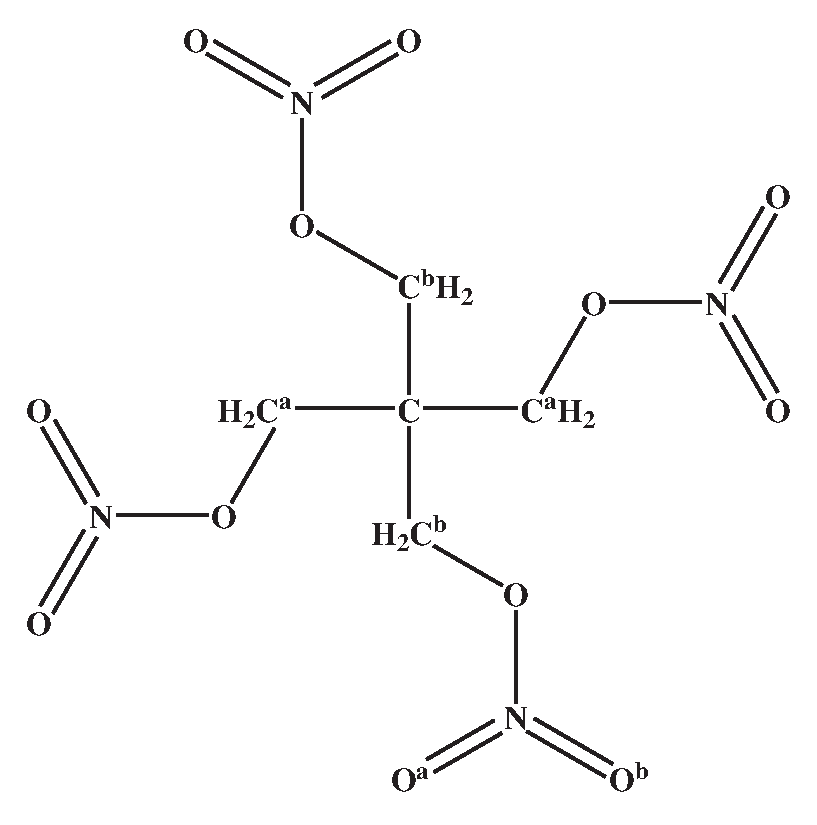
\includegraphics[clip]{petn_2d.eps}}
\caption{
Chemical structure of PETN.  Superscripts ``a'' and ``b'' are used
in Table~\ref{tab:table2} to distinguish geometrically distinct
internal coordinates for comparison to experiment.
}
\label{fig:petn_2d}
\end{figure}

\begin{figure}
\resizebox*{3.5in}{!}{\includegraphics[clip]{VRatio_EDiff_Press.eps}}
\caption{Volumetric hydrostatic compression for PETN.
(a) Energy difference $\Delta E$. The solid line is a sixth degree
polynomial fit to the $1\times 1\times 1$ predictions.  Crosses are
calculations for a $1\times 1\times 2$ supercell, and indicate that
finite-size effects are minimal.  (b) Pressure-volume relationship
calculated from the fit in (a).  Uncertainties in the experimental
data of Olinger {\it et al.}~\cite{Olinger_1975v62} are comparable to 
the symbol sizes.  }
\label{fig:volume_compress}
\end{figure}

\begin{figure}
\resizebox*{3.5in}{!}{\includegraphics[clip]{CAndA.eps}}
\caption{Linear compression of PETN.  (a) Relative linear compression
of the lattice parameters. Squares and circles correspond to the $a$
and $c$ crystallographic axes, respectively; dashed lines are simply a
guide for the eye.  Experimental data from Olinger {\it et
al.}~\cite{Olinger_1975v62}; experimental uncertainties are comparable
to the size of the symbols. (b) Ratio of $c$ to $a$.  Squares denote
calculated results; dashed line is a guide for the eye.  Circles are
experimental data;~\cite{Olinger_1975v62} error bars in $c/a$ and
$V/V_0$ are representative; solid line is a polynomial form taken from
Ref.~\cite{Olinger_1975v62}.  }
\label{fig:linear_compress}
\end{figure}

\begin{figure}
\resizebox*{3.5in}{!}{\includegraphics[clip]{VRatio_Bond_Angle_CloseContact.eps}}
\caption{(a) Variation of bond lengths in PETN as a function of hydrostatic 
compression.  Circle: C-C; square: C-O; diamond: O-N; up-triangle and
cross: N=O; down-triangle and plus: C-H.  (b) Variation of
three-center angles. Circle: C-C-C; square: C-O-N; diamond: C-C-H;
up-triangle: H-C-O; cross: C-C-O. (c) Compression of intermolecular
van der Waals 
contacts whose value is less than 3 \AA\/ at zero pressure.  All three
correspond to O$\cdot\cdot\cdot$H contacts.}
\label{fig:intramolecular}
\end{figure}
\end{document}
